%------------------------------------------------------------
%     
%     T H E S I S   T E M P L A T E   F O R   T H E 
%
%          U N I V E R S I T Y   O F   Y O R K
%
%------------------------------------------------------------
%
%  Written by Luke Abraham May 2006
%
%  The Author found this template suitable for the submission
%  of a Ph.D. Thesis in Dec 2006 (final submission May 2007).
%  Any changes to the regulations since then may render this 
%  template invalid - please consult
%
%     http://www.york.ac.uk/admin/gso/thesis.htm
%     http://www.york.ac.uk/admin/gso/binding.htm
%
%  for current guidelines
%
%  The author submitted his degree in Physics, so the 
%  template is designed for maths-heavy subjects.
%  The author also recommends the use of SUBVERSION as a
%  version repository system to maintain thesis updates.
%
%    http://subversion.tigris.org/
% 
%  I have also included a Makefile which contains the handy
%  LaTeX commands and is suitable for use on the Linux/Unix
%  system.
%
%  With thanks to Maff Glover, Josh Uretsky and Iain Hall
%  for useful additions to this template
%
%------------------------------------------------------------

% York is one sided in most situations
\documentclass[12pt,a4paper,onesided]{report}

% Use the following to selectively exclude chapters
%\includeonly{cover,abstract,acknowledge,declare,chapter1,chapter2}

% Package for figures
\usepackage[dvips]{graphicx}
\usepackage{fancyhdr}
\usepackage{setspace}
\usepackage{mathptmx}

% packages for maths symbols
\usepackage{amsmath}
\usepackage{amsmath} 
\usepackage{amsbsy}
\usepackage{amsthm}
\usepackage{amssymb}
\usepackage{amsfonts}
% algorithm package
\usepackage{algorithm}
\usepackage{algorithmic}
% allows for color - probably not needed
\usepackage{color}
% allows for three-part tables
\usepackage{threeparttable}
% extra maths scripts - could cause problems on older tetex installs
\usepackage[mathscr]{euscript}
\usepackage{eufrak}
\usepackage{bbold}

% font stuff - at the time of writing the offical University font is
% Palatino, hence its use here! 
\usepackage[T1,OT1]{fontenc}
\usepackage{palatino}
% other fonts
%\usepackage{times}
%\usepackage{bookman}
% uses paltino font with CM mathematics
%\usepackage{palatcm}

% underlining
\usepackage[normalem]{ulem}

% random stuff copied from elsewhere that I can't really 
% remember what it does - best to leave it alone
  \makeatletter
  \def\@dotsep{4.5}
  \makeatother

% increases the column seperation in tables (I think)
\setlength{\tabcolsep}{5pt}

% new definition of a space for typesetting
\newlength{\myVSpace}
\setlength{\myVSpace}{1ex}
\newcommand\xstrut{\raisebox{-.5\myVSpace}
  {\rule{0pt}{\myVSpace}}
}
\addtolength{\myVSpace}{10pt}

% handy math macros
\newcommand{\dif}{\mathrm{d}}
\def\dbar{{\mathchar'26\mkern-9mu \mathrm{d}}}
\newcommand{\Ang}{\mbox{\AA}}
\newcommand{\ev}{\mbox{eV}}
\newcommand{\ma}{\mbox{a}}
\newcommand{\mb}{\mbox{b}}

% use natbib package - it is the best - BUT, remember the syntax
% for full functionality
% use \citep{} for (ref (Year))
% and \citet{} for ref (Year)
% see documentation for more information
\usepackage[square]{natbib}

% use the 'geometry' package to setup page margins easily  :-)
% THESE ARE THE UNIVERSITY MARGINS
\usepackage[left=4.0cm,top=2.5cm,right=2.5cm,bottom=2cm,footskip=1cm]{geometry} 

%% Various parameters
%\setlength{\textheight}{229mm}
%\setlength{\topmargin}{-5.4mm}
%\setlength{\textwidth}{150mm}
%\setlength{\oddsidemargin}{14.6mm}
%\setlength{\evensidemargin}{14.6mm}
%% fix annoying right margin
%\addtolength{\oddsidemargin}{-1.0cm}

\setcounter{secnumdepth}{3}
\setcounter{tocdepth}{4}


% remove indentation from start of paragraphs
\setlength{\parindent}{0pt}

% gap between paragraphs
\setlength{\parskip}{5pt}

% ONE AND A HALF LINE SPACING
\onehalfspacing

\begin{document}
% page numbers are 1, 2 etc.
\pagenumbering{arabic}
%%%%%%%%%%%%%%%%%%%%%%%%%%%%%%%%%%%%%%%%%%%%%%%%%%%%%%%%%%%%%%%%%%%%%%%%%%%%%%%%
% This is the template for the title page. Please feel free to edit it to suit
% your needs, but please DO NOT HARDCODE YOUR NAMES and USE THE COMMANDS
% PROVIDED BY THE CLASS!!!
%%%%%%%%%%%%%%%%%%%%%%%%%%%%%%%%%%%%%%%%%%%%%%%%%%%%%%%%%%%%%%%%%%%%%%%%%%%%%%%%

\makeatletter                           % Make @ a simple letter
\singlespacing

\begin{titlepage}                       % Initialize titlepage environment
\newgeometry{                           % Change the default geometry
    right=1.8cm, left=1.8cm,            %
    top=2.0cm, bottom=2cm,              %
}                                       %

\newlength{\titlewidth}
\setlength{\titlewidth}{.95\textwidth}

\begin{minipage}[]{65mm}
    \raggedright                        % identifier according to the
    
\includegraphics[                   % regulations. Please do not edit its
        width=65mm]{CUnibig.eps}        % dimensions
\end{minipage}                          %
\hfill
\begin{minipage}[]{15mm}       % Here the crest and the name of the
    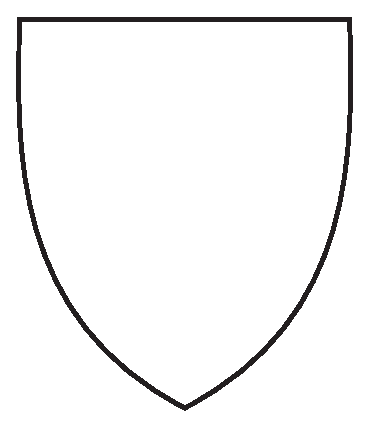
\includegraphics[width=13mm]{empty} % font and make other adjustments if you
\end{minipage}                          % how to fix it.
\pbox[m]{52mm}{\LARGE\college}                      % like. However, make sure, that you

\onehalfspacing                         % Switch to 1.5 spacing as it looks the 
                                        % best for titles, authors and similar
                                        % stuff

\centering\vfill\vfill                  % Center and insert 2x white space

\begin{minipage}[c]{\titlewidth}        %
    \centering\huge                     %
    \@title\vspace{5mm}                 %
\end{minipage}                          %

\vfill                                  % Insert white space

\begin{minipage}[c]{.6\titlewidth}      %
    \raggedright\large                  %
    \begin{tabular}                     %
        {>{\it}p{.4\textwidth}          %
         >{\raggedleft}p{.6\textwidth}} %
        Author: & \@author              %
        \tabularnewline                 %
        Supervised by: 
        &
        \pbox[t]{.6\textwidth}{\supervisor}    %
    \end{tabular}                       %
\end{minipage}                          %

\vfill                                  % Insert white space

\begin{minipage}[c]{.8\textwidth}       %
    \centering                          %
    \large\textit{\@subtitle}           %
    \\\@date                            %
\end{minipage}                          %
\end{titlepage}                         %

\defaultspacing                         % Return to default line spacing
\restoregeometry                        % Return to the default geometry
\makeatother                            
\setcounter{page}{1}

% Editor settings
% vim: tw=80
          % This is the front page
\addcontentsline{toc}{chapter}{\numberline { }Abstract}
\pagestyle{plain}
%\pagenumbering{roman}
\setcounter{page}{2}

\begin{center}
    {\LARGE\bf Abstract}
\end{center}

This thesis rocks! Need I say more...

\newpage

       % Apstract
\addcontentsline{toc}{chapter}{\numberline { }Contents}
\tableofcontents
% list of figures, tables etc - will then be added to table of contents
\listoffigures
\addcontentsline{toc}{chapter}{\numberline { }List of Figures}
\listoftables
\addcontentsline{toc}{chapter}{\numberline { }List of Tables}
% add list of algorithms if needed
\listofalgorithms
\addcontentsline{toc}{chapter}{\numberline { }List of Algorithms}
\addcontentsline{toc}{chapter}{\numberline { }Declarations}
\pagestyle{plain}

\begin{center}
    {\LARGE\bf Declarations}
\end{center}

I declare that the work presented in this thesis, except where otherwise stated,
is based on my own research and has not been submitted previously for a degree
in this or any other university. Parts of the work reported in this thesis have
been published in:

\begin{trivlist}
\item {\bf You and Your Supervisor}, ``A Very Interesting Paper'', \emph{Your Fav. J.} {\bf Vol}, Page
\item {\bf You, Your Supervisor and Another Person}, ``Another Very Interesting Paper'', \emph{Your Fav. J.} {\bf Vol}, Page
\end{trivlist}
\ \\ \ \\ \ \\ \ \\ \ \\ \ \\ \ \\ \ \\ \ \\ \ \\ 
Signed
\\ \ \\ \ \\ \ \\ \ \\ 
Your Name

\newpage
        % (optional) - declarations of previous papers
\addcontentsline{toc}{chapter}{\numberline { }Acknowledgements}
\pagestyle{plain}

\begin{center}
    {\LARGE\bf Acknowledgements}
\end{center}


I'd like to thank the men in the white coats who give me the little yellow pills, 
and the pink elephants, who keep me sane.

 % Acknowledgements
\newpage

% now set up what pages look like
\pagestyle{fancy}
\fancyhead[L]{\textsl{\chaptername\ \thechapter}}
\fancyhead[R]{\textsl{\leftmark}}
\fancyfoot[C]{\thepage}
\renewcommand{\headrulewidth}{0.4pt}
\renewcommand{\chaptermark}[1]{\markboth{#1}{}}


% include the chapters - these are contained in the sub-directories
\chapter{Introduction}

This is the introduction and I can say a lot about it.

Haha, this is a very long introduction.

\section{First section}

aksdjlasjdalksjdalksjdaslkdjas

\chapter{Not Introduction}

This is the introduction and I can say a lot about it.

\pagestyle{fancy}


\chapter{Chapter 3}


\section{Second Section}


\subsection{Second Sub-Section}


\subsubsection{Second Sub-Sub-Section}

I wouldn't bother looking at figure \ref{fig:very_dull_again}.

\begin{figure}[b]
\begin{center}
\includegraphics*[scale=1.0]{chap2/temp.eps}
\end{center}
\caption[Another dull figure.]{Another very boring figure from \citet{lukeabraham.com}.} 
\label{fig:very_dull_again}
\end{figure}


\chapter{Things}

More dummy text.

\pagestyle{fancy}


\chapter{Chapter 5}


\pagestyle{fancy}


\chapter{Chapter 6}

\pagestyle{fancy}


\chapter{Conclusions}


I found out stuff. It was great.

% put in the appendix
\appendix
% need to change ``Chapter A'' to ``Appendix A''
\renewcommand{\chaptername}{Appendix}
\chapter{Recipe for Cinnamon Balls}
\label{app:cinball}

\begin{table}[h]
\centering
\begin{tabular}{c|c}
\hline
\hline
\textbf{Ingredient}           & \textbf{Amount}  \\
\hline
egg whites                    & 2                  \\                
Castor (superfine) sugar      & 100\,g (4\,oz / $\frac{1}{2}$\,cup) \\
ground almonds       	      & 200\,g ($1/2$\,lb / 2\,cups)      \\ 
cinnamon		      & 1 level tablespoon         \\        
icing (confectioners') sugar  & (approx 5mm deep in a plate or wide bowl)\\    
\hline      
\end{tabular}
\end{table}        

\begin{algorithm}[h]
\begin{algorithmic}[1]
\STATE Beat the egg whites till they form stiff peaks.
\STATE Fold in all the remaining ingredients.
\STATE Form into balls with wetted hands.
\STATE Bake on a greased tray at $170^{\circ}$\,C (Gas Mark 3 / $325^{\circ}$\,F) for 25 minutes, or until just firm to the touch.
\STATE Roll in icing sugar whilst warm.
\STATE Roll in icing sugar when cold.
\end{algorithmic}
\caption[Recipe for Cinnamon Balls.]{The Perfect Cinnamon Balls \cite{Rose04}}
\end{algorithm}

I find it easier to mix the dry ingredients first, before adding them to the egg whites. This ensures a more even mixing.

It is important to bake the balls only as long as directed to ensure that the biscuits remain soft and moist inside. 
It may seem that they are still underdone, but it is important that they are not allowed to dry out.

These amounts make about 15-20 depending on the size of the cinnamon balls. 
I find it best {\em not} to pre--heat the oven otherwise they may burn. 
Also use a clean baking sheet, or one that has only been used for 
cakes/biscuits, to improve taste. Remove them from the baking sheet with a firm twist, or a thin spatula.

It is also possible to replace cinnamon with the contents of a vanilla pod and a tea-spoon of
vanilla essence, to make Vanilla Balls!


%\fancyhf
\fancyhead[L]{\textsl{}}
\fancyhead[R]{\textsl{\leftmark}}
\fancyfoot[C]{\thepage}
\renewcommand{\headrulewidth}{0.4pt}
% include the bibliography
\bibliographystyle{refs/plainnat}
\renewcommand{\chaptermark}[1]{\thechapter{#1}{}}
\addcontentsline{toc}{chapter}{\numberline { }Bibliography}
% need to change ``Chapter'' to ``Bibliogoraphy''
\renewcommand{\chaptername}{Bibliography}
\bibliography{refs/thesis.bib}

\end{document}
